\documentclass{article}
\usepackage[utf8]{inputenc}
\usepackage[table]{xcolor} % For cell coloring
\usepackage{geometry} % For page margins
\usepackage{graphicx} % For including images
\usepackage{float} % For image placement
\usepackage{tabularx} % For table stretching
\usepackage{multirow}
\usepackage{colortbl}
\usepackage{xspace}
\usepackage{hyperref}
\usepackage{parskip}
\usepackage{amsmath}

\usepackage{listings}


\usepackage{titlesec}
\titleformat{\subparagraph}
    {\normalfont\normalsize\bfseries}{\thesubparagraph}{1em}{}
\titlespacing*{\subparagraph}{\parindent}{3.25ex plus 1ex minus .2ex}{.75ex plus .1ex}


\input{/home/oddish3/Documents/uni/mast-2/preamble.tex}
\input{/home/oddish3/Documents/uni/mast-2/notation.tex}

% Moment Test and Descriptive Statistics
\newcommand{\amu}{0.10\xspace}
\newcommand{\asigma}{1.83\xspace}
\newcommand{\askew}{-0.32\xspace}
\newcommand{\akurt}{4.26\xspace}
\newcommand{\amut}{0.83\xspace}
\newcommand{\askewt}{-2.08\xspace}
\newcommand{\akurtt}{4.06\xspace}
\newcommand{\ajbt}{20.85\xspace}
\newcommand{\amup}{0.40\xspace}
\newcommand{\askewp}{0.04\xspace}
\newcommand{\akurtp}{0.00\xspace}
\newcommand{\ajbp}{0.00\xspace}

% Ljung-Box Test Results
\newcommand{\aistat}{27.06\xspace}
\newcommand{\aip}{0.17\xspace}
\newcommand{\aiistat}{25.61\xspace}
\newcommand{\aiip}{0.22\xspace}

% GARCH(1,1) with zt ~ N(0,1)
\newcommand{\bw}{2.53\xspace}
\newcommand{\ba}{0.13\xspace}
\newcommand{\bb}{0.15\xspace}
\newcommand{\bpi}{0.54\xspace}
\newcommand{\bpii}{0.03\xspace}
\newcommand{\bpiii}{0.90\xspace}

% GARCH(1,1) with zt ~ tv
\newcommand{\bwi}{0.24\xspace}
\newcommand{\bai}{0.07\xspace}
\newcommand{\bbi}{0.87\xspace}
\newcommand{\bvi}{4.62\xspace}
\newcommand{\bpti}{0.58\xspace}
\newcommand{\bptii}{0.22\xspace}
\newcommand{\bptiii}{0.00\xspace}
\newcommand{\bptiv}{0.00\xspace}

% GJR-GARCH(1,1) with zt ~ N(0,1)
\newcommand{\bwii}{3.06\xspace}
\newcommand{\baii}{0.00\xspace}
\newcommand{\bbii}{0.00\xspace}
\newcommand{\bgii}{0.29\xspace}
\newcommand{\bpgi}{0.02\xspace}
\newcommand{\bpgii}{1.00\xspace}
\newcommand{\bpgiii}{1.00\xspace}
\newcommand{\bpgiv}{0.19\xspace}

% GJR-GARCH(1,1) with zt ~ tv
\newcommand{\bwiii}{0.22\xspace}
\newcommand{\baiii}{0.02\xspace}
\newcommand{\bbiii}{0.89\xspace}
\newcommand{\bgiii}{0.07\xspace}
\newcommand{\bviii}{4.57\xspace}
\newcommand{\bpgtp}{0.26\xspace}
\newcommand{\bpgtpi}{0.57\xspace}
\newcommand{\bpgtpii}{0.00\xspace}
\newcommand{\bpgtpiii}{0.13\xspace}
\newcommand{\bpgtpiv}{0.00\xspace}

% residuals and squared lbq
\newcommand{\zone}{12.80\xspace}
\newcommand{\pone}{0.92\xspace}
\newcommand{\zfive}{16.87\xspace}
\newcommand{\pfive}{0.72\xspace}
\newcommand{\ztwo}{12.39\xspace}
\newcommand{\ptwo}{0.93\xspace}
\newcommand{\zsix}{16.21\xspace}
\newcommand{\psix}{0.76\xspace}
\newcommand{\zthree}{13.09\xspace}
\newcommand{\pthree}{0.91\xspace}
\newcommand{\zseven}{18.23\xspace}
\newcommand{\pseven}{0.63\xspace}
\newcommand{\zfour}{13.04\xspace}
\newcommand{\pfour}{0.91\xspace}
\newcommand{\zeight}{17.85\xspace}
\newcommand{\peight}{0.66\xspace}

% root mean square forecast error and dm test
\newcommand{\rmsfei}{1.16\xspace}
\newcommand{\rmsfeii}{1.10\xspace}
\newcommand{\rmsfeiii}{1.23\xspace}
\newcommand{\rmsfeiv}{1.11\xspace}
\newcommand{\dm}{0.84\xspace}
\newcommand{\dmpii}{0.72\xspace}
\newcommand{\dmi}{-0.94\xspace}
\newcommand{\dmpiv}{0.26\xspace}
\newcommand{\dmii}{0.75\xspace}
\newcommand{\dmpv}{0.70\xspace}


% Define colours
\definecolor{headercolor}{RGB}{169,169,169} % Grey color, adjust the RGB values as per your document
\definecolor{rowcolor}{RGB}{255,255,255} % White color, adjust if your document has a different row color

% Set page margins
\geometry{left=25mm,right=25mm,top=25mm,bottom=25mm}

% Custom column type for tabularx
\newcolumntype{Y}{>{\centering\arraybackslash}X}

\title{ECON60332 Coursework Template}
\author{Group 11} % INSERT GROUP NUMBER HERE
\date{}

\begin{document}

\maketitle

\noindent\begin{tabularx}{\linewidth}{|Y|Y|}
    \hline
    \rowcolor{headercolor} Participant’s Student ID & Indicate if the student did not participate \\
    \hline
    \multicolumn{1}{|c|}{10710007}\\
    \hline

\end{tabularx}

\section*{Theoretical exercise}

\subsection*{Question a}

When comparing the ARCH(2) model : $\sigma^2_{t} = \omega + \alpha_1 \epsilon_{t-1}^2 + \alpha_2 \epsilon^2_{t-2})$ to a GARCH(1,1)) : $\sigma^2_{t} = \omega + \alpha_1 \epsilon_{t-1}^2 + \beta_2 \sigma^2_{t-1})$

The following similarities emerge :
\begin{itemize}
	\item Both models capture the cluster effect where periods of high (low) volatility are followed by periods of high (low) volatility (probabilistically) 
		\item Both model capture overkurtosis, accounting for a heavier tail distribution than the standard norm
		\item If $z_{t}$ is not symmetric, then $\cov(\epsilon_t, \sigma^2_{t+1} | \ensuremath{\mathcal{F}}_{t-1})$ would not be zero, and both model are able to capture leverage (asymmetric) effects 
\end{itemize}

Though with key differences that
\begin{itemize}
	\item An arch model implies an AR model for the squared residuals whilst a GARCH model implies an ARMA model in both squared residuals and variance
	\item Fir the GARCH model $b_1$ can be unidentified if $a_1=0$
\end{itemize}

\subsection*{Question b}

Assuming $\alpha_1 + \alpha_2 < 1$ for stationarity

Where \( \mathcal{F}_{t-1} \) is the past history of the process, then the conditional expectation of \( \epsilon_t \) is given by:
\begin{equation}
	E(\epsilon_t | \mathcal{F}_{t-1}) = E(\sqrt{\sigma^2_t } z_{t}| \mathcal{F}_{t-1}) = \sigma_t E(z_t | \mathcal{F}_{t-1}) = \sigma_t \cdot 0 = 0
\end{equation}
Using LIE, we can obtain the unconditional mean :
\begin{equation}
E(\epsilon_t) = E(E(\epsilon_t | \mathcal{F}_{t-1})) = E(0) = 0
\end{equation}

To derive the second moment, we can express \( \epsilon_t^2 \) as an AR(22)-process:

\begin{align*}
\sigma^2_t + \epsilon^2_{t} = \omega + \alpha_1 \epsilon_{t-1}^2 + \alpha_2 \epsilon_{t-2}^2 + \epsilon^2_{t} \\
\epsilon_t^2 = \omega + \alpha_1 \epsilon_{t-1}^2 + \alpha_2 \epsilon_{t-2}^2 + \nu_t
\end{align*}
with \( \nu_t = \epsilon_t^2 - \sigma_t^2 \) being a WN process.

It holds that:
\begin{equation}
E(\epsilon^2_t | \mathcal{F}_{t-1}) = E(\sigma^2_t  z^2_{t}| \mathcal{F}_{t-1}) = \sigma^2_t E(z^2_t | \mathcal{F}_{t-1}) = \sigma^2_t \cdot 1 = \sigma^2_t
\end{equation}

Such that:
\begin{equation}
E(\nu_t | \mathcal{F}_{t-1}) = E(\epsilon_t^2 | \mathcal{F}_{t-1}) - \sigma_t^2 = \sigma_t^2 - \sigma_t^2 = 0
\end{equation}

Therefore:
\begin{equation}
E(\nu_t) = E(E(\nu_t | \mathcal{F}_{t-1})) = E(0) = 0
\end{equation}

Which allows us to write:
\begin{align*}
E(\epsilon_t^2) = \omega + \alpha_1 E \left[   \epsilon_{t-1}^2 \right] + \alpha_2  E \left[ \epsilon_{t-2}^2 \right] + E \left[ \nu_t \right] \\
&= \omega + \alpha_1 E \left[ \epsilon_{t-1}^2 \right] + \alpha_2  E \left[ \epsilon_{t-2}^2 \right]
\end{align*}

Using stationarity, \( E(\epsilon_{t-1}^2) = E(\epsilon_t^2) \) and hence we conclude that:

\begin{align*}
\mathrm{Var}(\epsilon_t) = E(\epsilon_t^2) - (E(\epsilon_t))^2 = E(\epsilon_t^2) =  \omega + \alpha_1 \mathrm{Var}(\epsilon_{t-1}) - \alpha_2 \mathrm{Var}(\epsilon_{t-2}) = \frac{\omega}{1- \alpha_1 - \alpha_2} = \frac{\omega}{1 - \sum_{i=1}^{2} \alpha_{i} } 
\end{align*}

\subsection*{Question c}

Using the covariance definition $\text{Cov}(X, Y) = E[XY] - E[X]E[Y]$ and given the conditional variance $\sigma^2_{t+1} = \omega + \alpha_1 \epsilon_{t}^2 + \alpha_2 \epsilon^2_{t-1}$, we derive the covariance as follows:
\begin{align*}
\text{Cov}(\sigma^2_{t+1}, \epsilon_t | \mathcal{F}_{t-1}) &= E[\sigma^2_{t+1} \epsilon_t | \mathcal{F}_{t-1}] - E[\sigma^2_{t+1} | \mathcal{F}_{t-1}]E[\epsilon_t | \mathcal{F}_{t-1}] \\
&= E[\sigma^2_{t+1} \epsilon_t | \mathcal{F}_{t-1}] - 0 \\
&= E \left[ \left( \omega + \alpha_1 \epsilon_{t}^2 + \alpha_2 \epsilon^2_{t-1} \right) \epsilon_t | \mathcal{F}_{t-1} \right] \\
&= \omega E[\epsilon_t | \mathcal{F}_{t-1}] + \alpha_1 E[\epsilon_t^3 | \mathcal{F}_{t-1}] + \alpha_2 E[\epsilon^2_{t-1} \epsilon_t | \mathcal{F}_{t-1}] \quad \text{(since $\omega$ and $\epsilon^2_{t-1}$ don't depend on $\epsilon_t$}) \\
&= 0 + \alpha_1 E[\epsilon_t^3 | \mathcal{F}_{t-1}] + 0 \quad \text{(since $\epsilon_t$ is conditionally zero-mean and independent of $\epsilon_{t-1}$)}.
\end{align*}

Now, if we consider $\epsilon_t = \sigma_t z_t$ :
\begin{align*}
\text{Cov}(\sigma^2_{t+1}, \epsilon_t | \mathcal{F}_{t-1}) =
\alpha_1 E[\epsilon_t^3 | \mathcal{F}_{t-1}] &= \alpha_1 E[(\sigma_t z_t)^3 | \mathcal{F}_{t-1}] \\
&= \alpha_1 \sigma_t^3 E[z_t^3 | \mathcal{F}_{t-1}] \\
&= \alpha_1 \left( \omega + \alpha_1 \epsilon_{t}^2 + \alpha_2 \epsilon^2_{t-1} \right)^\frac{3}{2} E[z_t^3].
\end{align*}
Only with  non-zero third moment on $z_t$, is the model able to capture the leverage (asymmetric) effect.   
Since $z_t ~ \mathcal{N}(0,\,1)$ , the third moment is 0 and $\text{Cov}(\sigma^2_{t+1}, \epsilon_t | \mathcal{F}_{t-1}) = 0$ so the model cannot capture the leverage effect, which is the tendency for negative shocks to have a different impact on volatility than positive shocks.

\subsection*{Question d}

With our ARCH(2) model, the 1 step ahead forecast is : $\sigma^2_{t+1 | t}  = \omega + \alpha_1  \epsilon^2_{t}  + \alpha_2  \epsilon^2_{t-1}$

Analogously the 2 step ahead forecast, where we take expectation of $\epsilon_t^2$, and use the unit variance of $z_{t}$ to simplify 
\begin{align*}
\sigma^2_{t+2 | t}  = E_t \left[  \omega + \alpha_1  \epsilon^2_{t+1}  + \alpha_2  \epsilon^2_{t}  \right] =   \omega + \alpha_1  \sigma^2_{t+1|t}  + \alpha_2  \sigma^2_{t}  
\end{align*}

Similarly for the 3-step ahead forecast, following the same logic

 \begin{align*}
 	\sigma^2_{t+3 | t} = E_t \left[  \omega + \alpha_1  \epsilon^2_{t+2}  + \alpha_2  \epsilon^2_{t+1}  \right] =   \omega + \alpha_1  \sigma^2_{t+2|t}  + \alpha_2  \sigma^2_{t+1} \equiv E \left[ \sigma^2_{t+3} | F_{t} \right] 
 \end{align*}

\subsection*{Question e}

The news impact curve illustrates how a shock to \( \epsilon_{t-1} \) affects \( \sigma_t^2 \).

We derive the unconditional long-term variance \( \bar{\sigma}^2 \) assuming that \( E(\epsilon_t^2) \) at any point is equal to \( \bar{\sigma}^2 \). From the stationarity condition:
\begin{equation}
E(\epsilon_t^2) = \omega + \alpha_1 E(\epsilon_{t-1}^2) + \alpha_2 E(\epsilon_{t-2}^2).
\end{equation}
Given \( E(\epsilon_{t-1}^2) = E(\epsilon_{t-2}^2) = \bar{\sigma}^2 \), the equation simplifies to:
\begin{equation}
\bar{\sigma}^2 = \frac{\omega}{1 - \alpha_1 - \alpha_2}.
\end{equation}

The news impact curve for the ARCH(2) model is then set up as:
\begin{equation}
\sigma_t^2 = \omega + \alpha_1 \epsilon_{t-1}^2 + \alpha_2 \bar{\sigma}^2.
\end{equation}
With the most recent shock \( \epsilon_{t-1} \) highlighted, we rewrite it as:
\begin{equation}
\sigma_t^2 = A + \alpha_1 \epsilon_{t-1}^2,
\end{equation}
where \( A = \omega + \alpha_2 \bar{\sigma}^2 \)

Thus with an asymmetric distribution, we can derive the NIC as :

\begin{equation}
\text{NIC}(\epsilon_{t-1} | \sigma_{t-1}^2 = \sigma_Y^2) = \omega + \alpha_1 \epsilon_{t-1}^2 + \alpha_2 \sigma_Y^2.
\end{equation}

\section*{Practical exercise}
\subsection*{Question a}

\begin{table}[H]
\centering
\begin{tabular}{|l|c|c|c|c|}
\hline
\rowcolor{headercolor}
 & Sample moments & & Test statistic & P-value \\
\hline
Mean & \amu &   Mean & \amut & \amup \\
\hline
Standard deviation & \asigma &  Skewness & \askewt & \askewp \\
\hline
Skewness &  \askew & Kurtosis & \akurtt & \akurtp \\
\hline
Kurtosis & \akurt & JB & \ajbt & \ajbp \\
\hline
\end{tabular}
\end{table}

\subsection*{LBQ test results:}
\noindent\begin{tabularx}{\linewidth}{|Y|Y|Y|}
    \hline
    \rowcolor{headercolor} & Returns & Squared returns \\
    \hline
    Test statistic & \aistat & \aiistat \\
    \hline
    P-value & \aip & \aiip \\
    \hline
\end{tabularx}

\subsubsection*{Plot of Daily Log Returns}

\begin{figure}[H]
    \centering
    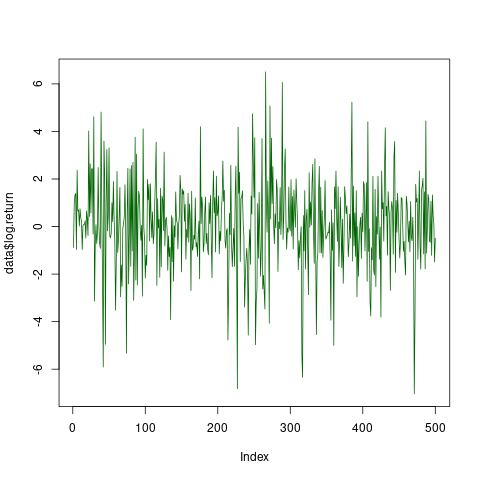
\includegraphics[width=0.35\textwidth]{../../docs/figures/log_return_plot.png}
    \caption{Log Return Plot}
    \label{fig:logreturn}
\end{figure}

\subsubsection*{SACF and SPACF}

\begin{figure}[H]
    \centering
    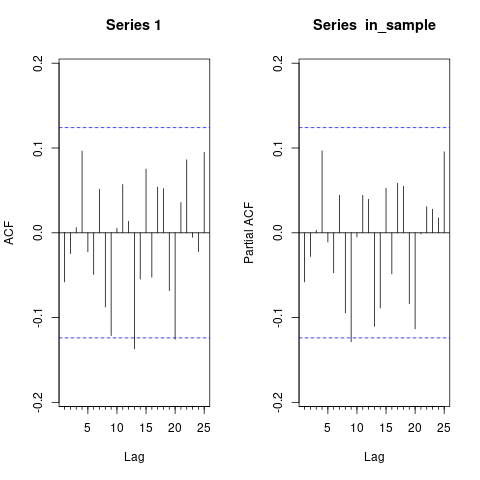
\includegraphics[width=0.35\textwidth]{../../docs/figures/PACF.png}
    \caption{Sample Autocorrelation and Partial Autocorrelation Function Plot}
    \label{fig:pacf}
\end{figure}

\subsection*{Interpretation}
Looking at the Descriptive Statistics, a skewness of \askew suggests there are more extreme negative returns than positive returns. 
Whilst a slightly higher kurtosis of \akurt suggests the distribution of returns has heavier tails and more extreme values.

Looking at the Test Statistics, testing mean returns are zero ($H_0 : \mu =0$ against $H_1 : \mu \neq 0$) with a one-sided test, we obtain a p-value of \amup, meaning we fail to reject $H_0$ at all conventional significance levels, we do not have enough evidence to conclude the mean return is zero. 

Testing the skewness of the return series is zero ($ H_1: \gamma = 0$ against $H_1 : \gamma \neq 0$) with a one-sided test, we obtain a p-value of \askewp and thus we reject the null hypothesis in favour of the alternative hypothesis that the distribution of returns is significantly skewed, and hence non-symmetric. 

Testing for the leptokurtic property in the returns ($H_0 : \kappa = 3$ against $H_1 : \kappa \neq 3 $) using a one-sided test, we obtain a p value of $\akurtp$, thus we reject the null hypothesis in favour of the alternative hypothesis that the returns have a significantly different kurtosis from 3, confirming the presence of heavy tails in the distribution. 

Using the Jargue-Bera test for normality ($H_0 : \gamma = 0 \& \kappa = 3$ against $H_0 : \gamma \neq 0 \& \kappa \neq 3$)  we obtain a p-value of \ajbp, thus we reject the null hypothesis in favour of the alternative hypothesis that the distribution of returns differs significantly from normality, as evidenced by the skewness and kurtosis. 

Using the LBQ test for the autocorrelation of the returns ($H_0: \rho_1 = \rho_2 = \ldots = \rho_{21} = 0$ against $H_1: \rho_i \neq 0$ for some $i \in \{1, 2, \ldots, 21 \}$), we obtain a p-value of 0.17 and 0.22 for the squared returns, hence we do not reject the null hypothesis at any conventional significance level, and thus there is no significant evidence of autocorrelation in the returns of the series.

Whilst the Daily Log-returns do not display a clear trend or seasonal pattern, though the volatility appears to be clustered in certain periods, indicative of heteroskedacity, there is no consistent pattern of significant lags in both the SACF and SPACF.
Though a significant negative correlation at lag 13 alongside lags approaching significance at 9 and 20 suggests some evidence for a seasonal pattern, however the presence of significant lags mainly inform us the time series is not white noise and exhibits some autocorrelation. 

\subsection*{Question b}

\begin{table}[H]
\centering
\begin{tabular}{|c|c|c|c|c|c|}
\hline
\rowcolor{gray!50}
\multicolumn{3}{|c|}{GARCH} & \multicolumn{3}{|c|}{GJR-GARCH} \\ 
\hline
Parameter & Estimate & P-value & Parameter & Estimate & P-value \\ 
\hline
$\omega$ & \bw & \bpi & $\omega$ & \bwii & \bpgi \\
\hline
$\alpha$ & \ba & \bpii & $\alpha$ & \baii & \bpgii \\
\hline
 $\beta$ & \bb & \bpiii & $\beta$ & \bbii & \bpgiii \\
\hline
GARCH-t & & & $\gamma$ & \bgii & \bpgiv \\
\hline
 $\omega$& \bwi & \bpti & GJR-GARCH-t &  & \\
\hline
 $\alpha$& \bai & \bptii & $\omega$ & \bwiii & \bpgtp \\
\hline
 $\beta$ & \bbi & \bptiii & $\alpha$ & \baiii & \bpgtpi \\
\hline
$\nu$ & \bvi & \bptiv & $\beta$ & \bbiii & \bpgtpii \\
\hline
& & & $\gamma$ & \bgiii & \bpgtpiii \\
\hline
& & & $\nu$ & \bviii & \bpgtpiv \\
\hline
\end{tabular}
\end{table}


\subsubsection*{Interpretation:}

For the GARCH model, a significant $\beta$ at the 1\% level suggests past volatility is very important to current volatility, whilst a significant $\alpha$ at the 10\% level suggests lagged squared returns are important in current volatility under a standard normal distribution.  
Under a student-t distribution, the relationship on $\beta$ holds though $\alpha$ loses significance after the inclusion of $\nu$, which suggests heavy tails are important in the GARCH-t model, rather than lagged squared returns which may have been masking the effect under a normal distribution. 

For the  GJR-GARCH model, $\beta$ remains significant at the 1\% level, suggesting past volatility remains important to current volatility upon the inclusion of the asymmetric impact of shocks. 
Although a negative $\gamma$ suggests positive shocks to returns increase future volatility more than negative shocks. 
Still, the $\alpha$ parameter becomes less certain with a larger p-value
Under a student's t-distribution for the GJR-GARCH model, $\beta$ and $\nu$ are significant, indicating the presence of heavy tails in the data is signifiant that could be important in modelling the current variance when accounting for asymmetries. 
Since they are similar in magnitude to the GARCH-t model a distribution with heavier tails is motivated, whilst asymmetric effects are not in the data. 

\subsection*{Question c}
\subsubsection*{Plot of NIC}
 
\begin{figure}[H]
    \centering
    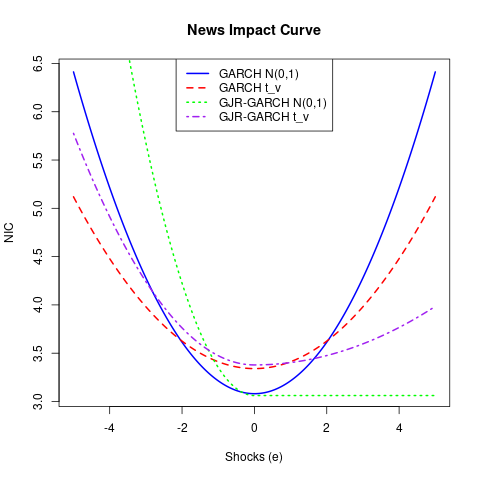
\includegraphics[width=0.35\textwidth]{../../docs/figures/NIC.png}
    \caption{News Impact Curve Plot}
    \label{fig:nic}
\end{figure}

\subsubsection*{Interpretation}


In \cref{fig:nic} we can see that the GJR news impact curve captures the asymmetry in the effect of news on volatility since it has a steeper slope on its positive side than its negative compared to the GARCH model which inherently does not capture the asymmetry.
The student's t-distribution in GJR-GARCH combines both the asymmetry of shocks (leverage effect) and the reduced impact of outliers, highlighting the importance of the leverage effect - properties which may enable better fitting of empirical returns.
Thus, in a market uptick like AN AI boom, under a GJR-GARCH-t model the impact of the asymmetry and heavy tails is more pronounced for the GJR-GARCH, so positive shocks to returns will increase future volatility more than negative shocks, which is counter to the usual leverage effect observed in financial markets. 

\subsection*{Question d}

\begin{table}[H]
\centering
\begin{tabular}{|l|c|c|}
\hline
\rowcolor{headercolor}
GARCH & Test statistic & P-value \\ 
\hline
Z & \zone & \pone \\ 
\hline
\(Z^2\) & \zfive & \pfive \\ 
\hline
\rowcolor{headercolor}
GARCH-t & Test statistic & P-value \\ 
\hline
Z & \ztwo & \ptwo \\ 
\hline
\(Z^2\) & \zsix & \psix \\ 
\hline
\end{tabular}
\quad % To add some spacing between the two tables
\begin{tabular}{|l|c|c|}
\hline
\rowcolor{headercolor}
GJR-GARCH & Test statistic & P-value \\ 
\hline
Z & \zthree & \pthree \\ 
\hline
\(Z^2\) &  \zseven & \pseven \\ 
\hline
\rowcolor{headercolor}
GJR-GARCH-t & Test statistic & P-value \\ 
\hline
Z & \zfour & \pfour \\ 
\hline
\(Z^2\) & \zeight & \peight \\ 
\hline
\end{tabular}
\end{table}

\subsubsection*{Interpretation:}

Though there are high p-values for the residuals across all models, indicating there is no statistical evidence to reject the null hypothesis that the residuals follow the respective distributions (and are thus white noise (normally distributed with no autocorrelation))

We are mainly interested in the p-values for the squared residuals to identify volatility clustering or ARCH effects
Accordingly, the model with the highest p-value for the square residuals is the GARCH-t model, indicating the least amount of autocorrelation is the GJR-GARCH-t. 
Though we would want to verify this with model selection criteria rather than a box test.

\subsection*{Question e}

\begin{table}[H]
\centering
\begin{tabular}{|l|c|c|c|c|}
\hline
\rowcolor{gray!50}
& GARCH & GARCH-t & GJR-GARCH & GJR-GARCH-t \\
\hline
RMSFE & \rmsfei & \rmsfeii & \rmsfeiii & \rmsfeiv \\
\hline
DM Test statistic & NA & \dm & \dmi & \dmii \\
\hline
P-value & NA & \dmpii & \dmpiv & \dmpv \\
\hline
\end{tabular}
\end{table}

\subsubsection*{Interpretation:}

Interpreting the results, the GARCH-t is the best model with the lowest RMSFE at 7.29. 
Although the Diebold-Mariano test suggests that the original GARCH model may have better forecast accuracy, with much higher p-values than conventional significance levels (e.g., 0.05 or 0.10), there's no statistical evidence that the forecast accuracy of GARCH-t and GJR-GARCH-t is any different from GARCH.

Empirically, this suggests that a more parsimonious, simpler GARCH model may have the edge over more complex models for forecasting this particular variance, as they do not provide statistically significant improvements in forecast accuracy.

\subsection*{Question f}
\subsubsection*{Interpretation:}

The choice of GARCH model involves a tradeoff between model misspecification and estimation noise. On one hand, simpler models like the standard GARCH have fewer parameters and are less prone to estimation noise, but may suffer from misspecification if the true volatility process exhibits features that the model cannot capture (e.g., asymmetry, time-varying volatility).

More flexible models like the GJR-GARCH or GARCH with a student's t-distribution (GARCH+) could potentially fit the data better by accounting for these complexities such as  positive leverage effects, and hence reducing misspecification. 
However, this requires estimating more parameters which inherently introduces greater estimation noise.

While complex models may offer an improved in-sample fit, there is no guarantee for this in out-of-sample forecasting due to the curse of dimensionality resulting in increased estimation noise. 
The benefits of reduced misspecification may be offset by the noise from estimating additional parameters, especially in small samples.

Ultimately, model selection criteria such as AIC and BIC should be used to inform the tradeoff between  model misspecification and estimation noise. 
By penalising overly complex models, Simple GARCH models are preferred since they are more stable when estimating and thus have less estimation noise.


\newpage
\section*{Appendix}

For reproduction of said script, see \url{https://github.com/oddish3/FE-CW/tree/master}

\lstinputlisting[language=R]{../../code/Script.R}




\end{document}

